\documentclass[a4paper,12pt]{article}
\usepackage{graphicx}
\begin{document}

\vspace*{\fill}
\centerline{\huge \textbf{Documentation}} \hspace*{\fill}
\vspace*{\fill}
\\
\tableofcontents
\newpage

\section{Introduction}
This web application is a forum of questions and answers, akin to \emph{stackoverflow} and \emph{yahoo answers}. The web service will let a user find solutions to problems either by browsing the web site or asking a question oneself. Questions can be answered by other users and each answer can be rated. Highest rated solution offers are shown at the top. With enough questions and answers in the database, the service can provide a quick and convenient way to look up a solution for a problem of any kind. Tags can be added to the asked question to help browsing questions by category.\\
\indent Service will be hosted on university's users-server via Tomcat. Code will be written in Java via NetBeans IDE. App will use PostgreSQL database. User's browser will not require other scripts or plug-ins.
\newpage

\section{General view of the application}
The following is an actor chart, followed with a description for each user and action.\\
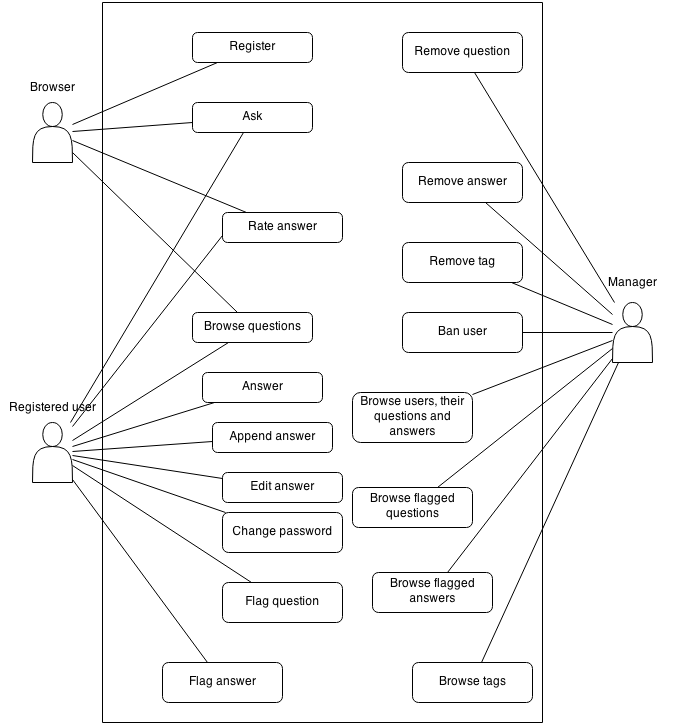
\includegraphics[scale=0.6]{ActorChart}

\noindent \textbf{Browser:} Unregistered user, that got access to the webapp simply by retrieving an url-link.\\
\textbf{Registered user:} User that has access to exclusive features by creating an account and logging into the app.\\
\textbf{Manager:} Webapp manager obligated to managing the forum, keeping it accessible to other users.\\

\noindent User actions:\\
\\
\textbf{Register:} Browser creates an account and promotes oneself into a registered user. User can then login to that account at any time if not banned.\\
\textbf{Ask:} User creates a question, awaiting a set of answers. Also sets tags for the question to improve the transparency of the question.\\
\textbf{Rate answer:} User marks answer as helpful and correct. Answer variant with most ratings is shown on top.\\
\textbf{Browse questions:} Lists questions by tags, (possibly a search function).\\
\textbf{Answer:} Adds an answer to a specified question.\\
\textbf{Append answer:} User edits one's answer by adding information into it. This way of editing will retain the rating of the answer.\\
\textbf{Edit answer:} User edits one's answer freely. This will reset the rating for the answer.\\
\textbf{Change password:} Registered user changes one's password.\\
\textbf{Flag question:} Notifies manager that specified question is inappropriate.\\
\textbf{Flag answer:} Notifies manager that specified answer is inappropriate.\\
\\
\textbf{Remove question:} Removes the specified question along with its answers.\\
\textbf{Remove answer:} Removes the specified answer.\\
\textbf{Remove tag:} Removes a tag from the database.\\
\textbf{Ban user:} Removes the user from the database. Questions and answers made by the user are either marked as 'banned', or removed completely.\\
\textbf{Browse users, their questions and answers}\\
\textbf{Browse flagged questions:} Lists questions by their amount of flags. Helps finding inappropriate questions.\\
\textbf{Browse flagged answers:} Lists answers by their amount of flags. Helps finding inappropriate answers.\\
\textbf{Browse tags:} Lists tags. Whether they are inappropriate or not is apparent directly from the tag.\\

\end{document}